Durch die optischen Besonderheiten von spiegelnd glänzenden Oberflächen werden solche in der Industrie an vielen Stellen verwendet.
Speziell in der Automobilindustrie werden täglich große Karosserieflächen glänzend lackiert.
Alleine in Deutschland wurden in den Jahren von 1990 bis 2021 im Durchschnitt ungefähr 5 Millionen Personenkraftwagen pro Jahr produziert \cite{statistaPKW}.
Ein großer Teil der Fahrzeuge erhalten nach der Lackierung eine spiegelnde Oberfläche.
Solche Oberflächen müssen durch besondere Verfahren auf Defekte überprüft werden.
Dabei sorgen spekulare Reflexionen dafür, dass die Oberflächen nicht direkt, sondern über ihre Spiegelbilder der Umgebung betrachtet werden müssen (siehe Abbildung \ref{img:spiegelndeKarosserie}).

% Abbildung: Beschriftung Delle
{
	\begin{figure}[H]
		\centering
		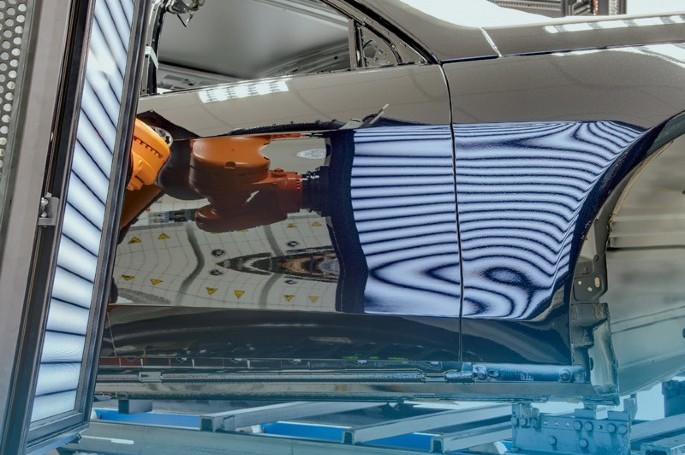
\includegraphics[width=0.5\textwidth]{01_einfuehrung/figures/spiegelndeKarosserie}
		\caption[Spiegelnde Karosserieoberfläche]{Spiegelnde Karosserieoberfläche \cite{spiegelndeKarosserieImg}}
		\label{img:spiegelndeKarosserie}
	\end{figure}
}

\noindent
Die riesige Menge an Oberflächen macht es für die Qualitätssicherung unumgänglich die Prüfung durch automatisierte Prozesse zu integrieren.
Dabei stoßen die üblichen Verfahren der industriellen Bildverarbeitung auf ihre Grenzen, sodass neue Methoden eingeführt werden müssen.
Diese speziellen Anwendungen erfordern den Einsatz von deflektometrischen Prüfaufbauten.
In der Industrie sind solche Verfahren schon seit Längerem zur Analyse der Topographie von spiegelnden Freiformflächen etabliert.
Deflektometrische Verfahren funktionieren nach einem ähnlichen Prinzip, wie auch die Inspektion von spiegelnden Oberflächen durch Menschen. 
Durch die Reflexionen und Verzerrungen auf glänzenden Oberflächen ist es möglich auf die Form und Krümmung der Oberfläche zu schließen.
Das wissenschaftliche Gebiet der Deflektometrie ist auch heute noch Thema für viele Forschungsarbeiten und wird stetig weiterentwickelt.

\p
Im Rahmen der Arbeit werden spekular reflektierende Objektoberflächen unter Projektion von bekannten Mustern durch eine Kamera aufgenommen, anschließend analysiert und auf Defekte überprüft.
Welche Informationen können aus der Beobachtung von Spiegelbildern gewonnen werden?
Wie sehen allgemein anwendbare Methoden aus, um spiegelnde Oberflächen erfolgreich zu bewerten?
Das Ziel der Arbeit ist es, diese Fragen zu erforschen und aufzuklären.
Des Weiteren sollen ein Aufbau, die Ansteuerung von Beleuchtung und Kamera und die notwendige Auswertung des Bildmaterials entwickelt werden, durch welche eine Erkennung von Oberflächendefekten ermöglicht wird.
Die Umsetzung soll dabei in Form einer Softwareerweiterung für NeuroCheck erfolgen, eines sogenannten \textit{Plug-ins}.

\p
Während der Arbeit soll außerdem ein bestimmter Sonderfall genauer betrachtet werden - transparente Prüfobjekte.
Die Problematik ist dabei, dass man neben der Reflexion des Lichts, mit der Transmission zu kämpfen hat.
Dafür gibt es verschiedene Lösungsansätze wie z. B. die Auftragung einer undurchsichtigen Beschichtung.
Eine andere Möglichkeit ist eine Veränderung in dem Prüfaufbau.
Anstatt ein Muster auf das Objekt zu projizieren, kann man eine Durchlichtbeleuchtung nutzen.
Das heißt, dass man auf einem Bildschirm unter dem transparenten Prüfobjekt verschiedene Muster anzeigt.

\p
Durch die aufgenommenen Muster können Aussagen über die Oberflächenbeschaffenheit getroffen werden.
Abhängig von den verwendeten Mustern und der Auswertung sollen damit bestimmte Fehlstellen kenntlich gemacht werden.
Als Fehlstellen gelten Verformungen und Oberflächendefekte wie z. B. Dellen, Kratzer oder matte Stellen.
%TODO Weiteres schreiben im Bezug auf die nachfolgende Arbeit (vermutlich eher gegen Ende)
%Zur Detektion dieser Defekte kann man verschiedene deflektometrische Verfahren einsetzen.
%Die Verfahren können verschiedene Ergebnisse liefern, abhängig davon sind eventuell aus den Ergebnissen weitere Verarbeitungen und Auswertungen nötig.
%Im Rahmen des Projektes werden speziell die deflektometrischen Verfahren betrachtet, welche für eine Vielzahl von Anwendungen genutzt werden können.
%Nachfolgende Verarbeitungen, z. B. Detektion von Zeichen und Kratzern, werden im Rahmen des Projekts und der Bachelor-Arbeit nicht genauer behandelt.